\chapter{Pruebas} \label{pruebas}

En este capítulo se describen las pruebas realizadas sobre los distintos microservicios que componen la aplicación, así como sobre el frontend. Estas pruebas serán esenciales para asegurar la calidad del software, detectar errores antes de llegar a estados más avanzados y garantizar un comportamiento estable. 

Además, se han integrado en el flujo de integración continua (CI) a través de las GitHub Actions, de manera que se ejecutan automáticamente en cada \textit{subida} a las ramas del repositorio. De este modo, las pruebas forman parte activa del ciclo de vida del desarrollo.

\vspace{0.5em}

Para cada componente se han definido distintos tipos de pruebas con el objetivo de cubrir tanto la lógica individual como el comportamiento global del sistema:

\begin{enumerate}
    \item \textbf{Pruebas Unitarias}: Verifican el comportamiento de clases y funciones de forma aislada, utilizando mocks para simular dependencias externas. Se emplean principalmente JUnit y Mockito para los servicios en Spring Boot, Pytest para los microservicios en Flask y Jest \cite{Jest} con React Testing Library para el frontend.
    
    \item \textbf{Pruebas de Sistema (End to End)}: Validan flujos completos que implican a varios componentes del sistema, especialmente los endpoints más críticos.
    
    \item \textbf{Pruebas de Widgets (Frontend)}: Evalúan la interacción de los elementos de la interfaz de usuario, garantizando su correcto comportamiento frente a las acciones del usuario.
\end{enumerate}

\section{Microservicio de Gestión de Usuarios}

\subsection{Pruebas Unitarias}
Se han probado los siguientes métodos de la capa de servicio:
\begin{itemize}
    \item \texttt{registrarUsuario(UserDTO dto)}: Verifica el registro de un nuevo usuario comprobando si el usuario o alguno de sus datos no han sido previamente registrados. En caso contrario, lanza una excepción controlada.
    \item \texttt{getUsuarioPorId(Long id)}: Comprueba la correcta recuperación de un usuario existente por ID. También se verifica el caso de error mediante una excepción.
    \item \texttt{getComunidadesGuardadas(Long userId)}: Comprueba que se recuperan correctamente las comunidades guardadas por un usuario, incluyendo el caso en que la lista esté vacía.
\end{itemize}

\subsection{Pruebas End to End}
\begin{itemize}
    \item \texttt{POST /user/login}: Se comprueba que con credenciales válidas se obtiene un JWT en la respuesta. También se prueba el caso de credenciales inválidas.
    \item \texttt{GET /user/\{id\}}: Verificación de que se devuelve la información del usuario correspondiente, y se maneja correctamente el caso de ID inexistente.
    \item \texttt{PUT /user/\{id\}}: Se prueba la actualización de datos del usuario y que los cambios se persisten correctamente en la base de datos.
\end{itemize}

Los test han sido pasados todos correctamente, cómo se puede ver en la imagen \ref{fig:test-result}
\begin{figure}[H]
  \centering
  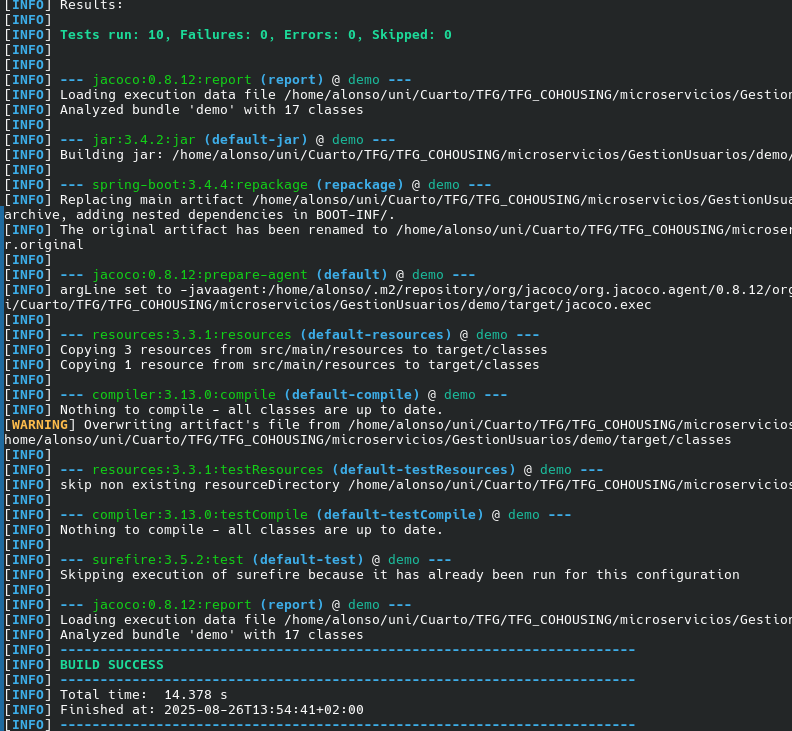
\includegraphics[width=1\textwidth]{fotos/resultadotest-micro-GestionUsuarios.png}
  \caption{Muestra del resultado de los test del microservicio Gestión de Usuarios}
  \label{fig:test-result}
\end{figure}
\section{Microservicio de Gestión de Comunidades}
Este microservicio contiene la lógica central del sistema, especialmente en cuanto a tareas colaborativas y reparto de responsabilidades.

\subsection{Pruebas Unitarias}
\begin{itemize}
    \item \texttt{encontrarPorNombre(String name)} y \texttt{encontrarPorId(Long id)}: Verificación de la recuperación correcta de comunidades por nombre o ID.
    \item \texttt{crearComunidad(CommunityDTO dto)}: Se prueba la creación de comunidades, validando que no exista ya una con el mismo nombre.
    \item \texttt{asignarTareasSemanales()}: Se comprueba que el algoritmo de reparto automático semanal de tareas se ejecuta de forma correcta y equilibrada.
    \item \texttt{addTareaAComunidad(Long communityId, TaskDTO dto)} y \newline \texttt{addEventoAComunidad(Long communityId, EventDTO dto)}: Validación de la correcta asociación de tareas y eventos a una comunidad.
\end{itemize}

\begin{lstlisting}[language=Java, caption={Pseudocódigo del test crearComunidad}]
test "crear comunidad" {
    // Creamos una comunidad falsa
    lifestyleDTO = new LifestyleDTO(1,1,1,1,1)
    dto = new CommunityDTO(
        id = 1L,
        name = "EcoWarning",
        description = "Comunidad preocupada con el medio ambiente",
        ownerId = 7L,
        lifestyle = lifestyleDTO,
        members = [1L, 4L],
        imageUrl = "https://foto",
        latitude = 40.423,
        longitude = 3.45,
        address = "Calle Falsa",
        price = 300.45,
        capacity = 2
    )

    // Mock: metodo para guardar la nueva comunidad 
    mock communityRepository.save(any Community)
        -> devuelve la misma Comunidad pasada

    // Probamos el metodo registrarComunidad
    comunidad = communityService.registrarComunidad(dto)

    // Comprobamos que la comunidad guardada tiene el nombre de la comunidad nueva registrada
    assert comunidad.getName() == "EcoWarning"
}
\end{lstlisting}
\subsection{Pruebas End to End}
\begin{itemize}
    \item \texttt{POST /community/\{id\}/unir}: Verifica que un usuario puede unirse correctamente a una comunidad.
    \item \texttt{GET /community/\{id\}/tasks}: Comprueba la obtención de tareas para su posterior planificación.
    \item \texttt{DELETE /community/\{id\}}: Se prueba la eliminación completa de una comunidad y la cascada de datos relacionada.
\end{itemize}

\section{Microservicio Recomendador}
Este microservicio ha sido implementado con Flask y probado mediante \texttt{pytest}.

\subsection{Pruebas Unitarias}
\begin{itemize}
    \item \texttt{obtener\_todas\_comunidades()}: Verifica que se recuperan correctamente todas las comunidades desde la base de datos.
    \item \texttt{get\_usuario\_perfil(user\_id)}: Prueba la obtención del perfil completo del usuario.
    \item \texttt{recomendar\_comunidades(UserDTO dto)}: Valida que el algoritmo de recomendación devuelve resultados coherentes según los intereses y preferencias del usuario.
\end{itemize}

\subsection{Pruebas End to End}
\begin{itemize}
    \item \texttt{GET /recomendaciones}: Comprueba que se devuelven comunidades recomendadas al usuario autenticado.
    \item \texttt{GET /recomendaciones-filtradas?filtro=\dots}: Se valida que los filtros personalizados funcionan correctamente y modifican los resultados retornados.
\end{itemize}


\begin{lstlisting}[language=Java, caption={Pseudocódigo del test recomendacionesFiltradas}]
test "recomendaciones filtradas" {
    // Se carga el usuario falso creado para las pruebas
    usuario = test_user
    user_id = usuario.id
    // Se define parametros de precio y distancia para el filtro
    parametros = {
        "precio": 400,
        "distancia": 5   # 5 km de radio
    }
    // Mock: get_usuario_por_id devuelve el usuario de prueba
    // Mock: get_comunidades_incompletas devuelve comunidades de prueba
    mock get_usuario_por_id -> usuario
    mock get_comunidades_incompletas -> test_communities

    // Se realiza la llamada al endpoint
    respuesta = client.get("usuarios/recomendaciones-filtradas/{user_id}", params=parametros)

    // Se realizan las comprobaciones de la respuesta del endpoint
    assert respuesta.status_code == 200
    datos = respuesta.json()
    assert len(datos) == 1                  // Solo una comunidad
    assert datos[0]["name"] == "Comunidad Cerca"
}
\end{lstlisting}

\section{Microservicio API Gateway}

\subsection{Pruebas Unitarias}
\begin{itemize}
    \item \texttt{extraerToken(HttpHeaders headers)}: Valida que el token JWT es correctamente extraído del encabezado \texttt{Authorization}.
    \item \texttt{validarToken(String token)}: Comprueba que el token es válido y no ha expirado.
\end{itemize}

\begin{lstlisting}[language=Java, caption={Pseudocódigo del test \texttt{validarToken} en \texttt{GatewayServiceTest}}]
test "validarToken" {
  // En primer lugar creamos un mock de los servicios que intervienen en la prueba
  mock JwtUtil, GatewayFilterChain, ServerWebExchange, ServerHttpRequest, ServerHttpResponse, HttpCookie
  
  cookie.value = "tokenValido"
  request.cookies["auth-token"] = cookie
  exchange.request = request
  exchange.response = response
  jwtUtil.validate("tokenValido") -> true
  chain.filter(exchange) -> empty

  // Realizamos la llamada al metodo a probar JwtAuthenticationFilter 
  result = JwtAuthenticationFilter(jwtUtil).filter(exchange, chain)

  // Comprobaciones finales
  expect(result).completes()
  verify(chain.filter(exchange)).calledOnce()
  verify(response.setComplete()).neverCalled()
}
\end{lstlisting}



\subsection{Pruebas End to End}
\begin{itemize}
    \item Se verifica que las peticiones entrantes se enrutan correctamente hacia los microservicios destino según el path y el método HTTP.
\end{itemize}

\section{Microservicio de Solicitudes}

\subsection{Pruebas Unitarias}
\begin{itemize}
    \item \texttt{getSolicitudesUsuario(Long userId)}: Valida que se obtienen todas las solicitudes activas del usuario.
    \item \texttt{deleteSolicitudes(Long userId)}: Prueba que se eliminan correctamente todas las solicitudes del usuario.
    \item \texttt{aceptarSolicitudUnion(Long solicitudId)}: Verifica el cambio de estado de la solicitud a Aceptada.
\end{itemize}
\begin{lstlisting}[language=Java, caption={Pseudocódigo del test aceptarSolicitudUnion}]
test "Aceptar Solicitud Union" {
    
    // Preparar datos de prueba
    solicitudId = 1
    solicitud = crearSolicitud(
        id = solicitudId,
        userOrigenId = 10,
        communityId = 20
    )

    // Mock: al buscar la solicitud, devolver el objeto creado
    mock(solicitudesRepository.findById(solicitudId)).returns(Optional.of(solicitud))

    // Ejecutar la funcion a probar
    response = solicitudesService.aceptarSolicitudUnion(solicitudId)

    // Verificar la respuesta HTTP
    assert response.statusCode == OK
    assert "Solicitud aceptada" en response.body

    // Verificar que se envio un mensaje a RabbitMQ
    verify(rabbitTemplate.convertAndSend(
        EXCHANGE_NAME,
        "comunidad.response",
        cualquierObjeto(UnionResponseDTO)
    ), veces=1)

    // Verificar que la solicitud fue eliminada del repositorio
    verify(solicitudesRepository.deleteById(solicitudId), veces=1)
}
\end{lstlisting}
\subsection{Pruebas End to End}
\begin{itemize}
    \item \texttt{GET /solicitudes/\{id\}}: Se obtiene la solicitud específica en función de Id.
    \item \texttt{GET /solicitudes/usuario/\{id\}}: Devuelve las solicitudes asociadas al usuario.
\end{itemize}


\section{Frontend}

Para las pruebas del frontend, desarrollado en \texttt{React} con \texttt{TypeScript}, se han utilizado las bibliotecas \texttt{React Testing Library} y \texttt{Jest}.

\subsection{Pruebas de Componentes}
\begin{itemize}
    \item Componente de comunidades recomendadas: Verifica que se renderizan correctamente los elementos y que los botones de acción funcionan como se espera.
    \item Componente de detalles de comunidad: Comprueba que los datos se cargan correctamente y que los botones permiten unirse o abandonar una comunidad.
    \item Panel de inicio: Se prueba la carga condicional del contenido según el rol del usuario (administrador, miembro) y su pertenencia a una comunidad.
    \item Solicitudes: Se valida que se visualizan y actualizan correctamente las solicitudes activas del usuario.
\end{itemize}

\begin{lstlisting}[language=Java, caption={Pseudocódigo del test de visualización y actualización de solicitudes}]
test "Mostrar Solicitudes"{
    
    // Mockear la API para devolver solicitudes de prueba
    mock(getSolicitudesUsuario(userId=123)).returns([
        { id: 1, tipo: "compleja", descripcion: "Solicitud de prueba 1" },
        { id: 2, tipo: "basica", descripcion: "Solicitud de prueba 2" }
    ])
    mock(aceptarSolicitud, rechazarSolicitud, eliminarSolicitud).returns({})

    // Renderizar la pagina con MemoryRouter
    render(SolicitudesPage, route="/solicitudes/123")

    // Comprobar que las solicitudes aparecen
    assert screen.findByText("Solicitud #1") exists
    assert screen.findByText("Solicitud de prueba 1") exists
    assert screen.findByText("Solicitud #2") exists
    assert screen.findByText("Solicitud de prueba 2") exists
}
test "Actualizar Solicitudes"{
    
    // Renderizar la pagina con MemoryRouter
    render(SolicitudesPage, route="/solicitudes/123")

    // Seleccionar y clickar el boton de actualizar
    updateButton = screen.getByRole("button", name="Actualizar solicitudes")
    fireEvent.click(updateButton)

    // Verificar que la primera solicitud sigue visible
    assert screen.findByText("Solicitud #1") exists
}
\end{lstlisting}
\section{Ejecución y Cobertura de Pruebas}
Gracias a la integración de las pruebas en el flujo de CI mediante GitHub Actions, estas se ejecutan automáticamente tras cada cambio. Como resultado:

\begin{itemize}
    \item Se asegura que cualquier modificación del código no rompa funcionalidades existentes.
    \item Se generan informes automáticos de cobertura de código mediante Codecov.
    \item Se garantiza que el desarrollo sigue un enfoque orientado a la calidad desde sus primeras etapas.
\end{itemize}

A continuación, se muestra una captura del informe de cobertura generado tras un merge exitoso a la rama \textbf{develop}, imagen \ref{fig:codecov}, se puede observar que el porcentaje de código cubierto tras los test realizados es del 42 por ciento. 

\begin{figure}[h!]
  \centering
  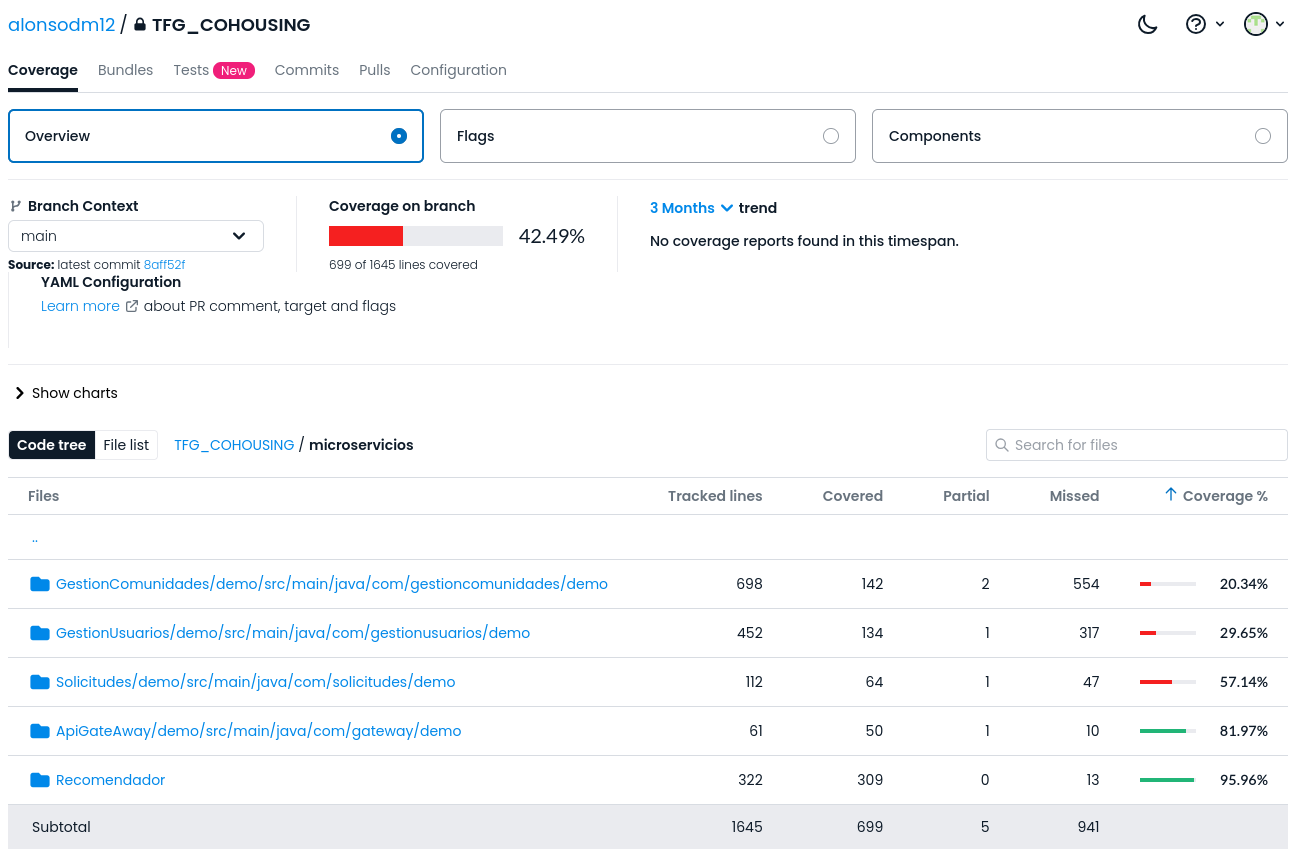
\includegraphics[width=1\textwidth]{fotos/codecov-coverage.png}
  \caption{Muestra del informe de cobertura por Codecov}
  \label{fig:codecov}
\end{figure}
